\begin{figure*}[t!]
\checkoddpage \ifoddpage \forcerectofloat \else \forceversofloat \fi
\frame{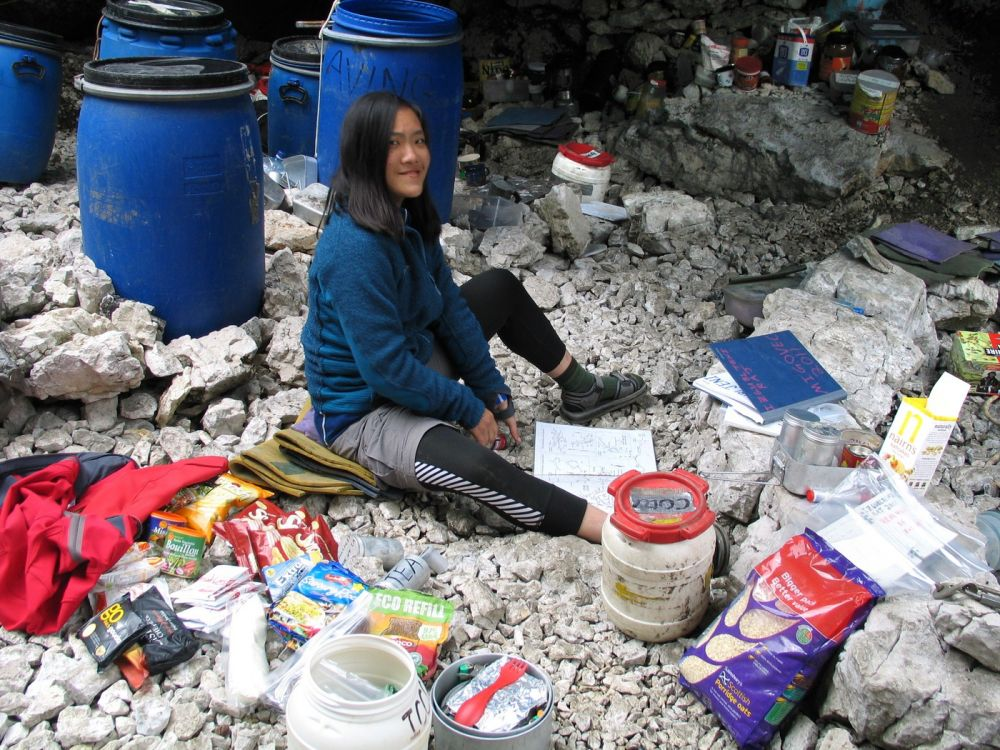
\includegraphics[width=\linewidth]{2011/stories/2011-07-20-12.21.54-Jarvist Frost-CanonG5-IMG_0111 - Preparing the first Underground Camp--orig_1050p.jpg}}
\caption{Clare Tan preparing provisions for the first overnight trip to underground camp. \pic{Jarvist Frost.}} \label{ug camp pack}
\end{figure*}



\section{Setting up camp: my first time in Vrtnarija!}


It was my first ever expedition and after three(?) days of carries in
rain and clag, I was eager to experience \passage{Vrtnarija} and alpine
caving firsthand. So when talk turned to plans for setting up
underground camp I made sure I was around for the conversation! It was
eventually decided that a team comprising myself, Jarv, Jan and Myles
would finish rigging down to camp, set up camp and spend a night there
before coming out the next day.

The morning was then spent on final preparations: packing the camp
tacklesacks, sorting out our provisions, grinding black pepper and
packing a cheeky set of survey instruments and bolting kit `just in
case'. Making our way across the plateau to the entrance, I was
admittedly feeling a little apprehensive. I'd never been that deep
underground before and had heard stories about the slog out from camp.
Was I overreaching myself by going down to camp on my first trip? I
trusted myself to make it out though, so it was with an air of
anticipation that I followed Myles into the cave.


\margininbox{Advice from the lags}{
Remember: If you stop pissing about in the bivvy and actually go caving, you'll be even more likely to find the connection. \mininame{Clewin Griffiths, via Facebook}}{\logbook}

Jarv went ahead to rig while the rest of us followed, each encumbered by
at least two bulky tacklesacks, stuffed with sleeping bags and assorted
camping equipment. We met Tetley and Jonny in the \passage{Urinal series},
on their way out from Tetley's traditional Mig fresher initiation to
\passage{Pico}/\passage{Swing}/\passage{Tessellator}.

\margininbox{21/7/2011 11:22 am}{

Camp is
5.3°C! Possibly due to the biological processes of the mould
civilisation controlling camp. Now for a little bimble and then out for
tea and medals. WOOF WOOF. \name{Myles}}{\logbook}

We made steady progress towards camp, chatting while waiting for Jarv to
rig, with Myles telling me about the pitches and where to look out for
loose rock. I like caving with old Myles. He exudes an aura of
confidence and competence. Whether that is true is another point
entirely.

Finally we made our way down \passage{Zimmer} and through \passage{Friendship
Gallery} to\ldots{} Camp \passage{X-Ray}! The overturned tent, courtesy of
DanG from last year's derig, greeted us. We set about making the camp
home: collecting sand to cover the mould which had multiplied in our 11
month absence, building the sleeping platform of rocks, and setting up
the beds of comf and sleeping bags. I was introduced to the delights of
underground cuisine and the luxury of clean, clean, fleecy comf to wear.
Less glamorous perhaps was having to piss into the same resealable bag
as Myles (I think? Check UG logbook! Or maybe this was in our
tent\ldots{})! I slept well that night.


\margininbox{Round Pond}{
     \begin{itemize}
    \item Jan Evetts
    \item Jarvist Frost
    \end{itemize}}{\explo}

The next morning after a brew Jan and Jarv decided to have a cheeky push
in \passage{Serpentine} before heading out, while I was to familiarise
myself with the cave with Myles. We pottered about \passage{Albert Hall}
and its various branches before finally heading down \passage{Serpentine}
to say hello to Jan and Jarv. We turned around at the bottom of \passage{It
Will Rain}, the 600 m of ascent on our minds. At this point Myles said
to keep going until \passage{Fistful of Tolars} as he'd be right behind me.
I headed out.

\margininbox{21/7 5pm}{\passage{Serpentine}/\passage{It will Rain}. Follow red rope down from \passage{Albert Hall}
-- at end of \passage{It will rain}, fairly difficult 1.5 m cascade/freeclimb to
start of pitch. We rigged \textasciitilde 5 m to ledge, look down 10-15
m (nice pitch!) into what appears to be chamber (big ish). With water.

Reheated tea and peanuts, time to head for surface! Good luck team Thursday/Friday!\name{Jarv}}{\logbook}

At \passage{Zimmer} I snagged a sneaky break, deciding to wait for
Myles\ldots{} and I waited, and waited, and waited. Just as I was
beginning to get concerned and go back for him, Myles appeared.
Apparently he'd got confused in \passage{Albert Hall} and had to try a few
passages before finding the right one back! A bit shaken but otherwise
fine, we made our bid for the surface at a steady pace. The prussick out
was actually less painful than I thought it would be; the never-ending,
one-foot-in-front-of-the-other slog associated with carries was good
preparation indeed!

We emerged to a smattering of rain but felt triumphant nonetheless. I
couldn't wait to go back!

\name{Clare Tan}

\newpage


\fullwidthbox{28/7/11 - Kate and Jan's underground camp}{My hands are extremely fucked so this may be short. Had a wonderful few days underground. Camp is as lovely as ever. I've even taken to eating
smash which I thought would never happen after the incident with the sleeping bag last year.

Had two pushing days, the first of which, despite Jan's heroic effort, was not so successful although we did answer the unanswered potential of the window off \passage{Cheetah}. Later that day after sitting at the top of \passage{Cheetah} freezing my bollocks off we went to find the location of the \passage{Red baron} and the pushing front where Clare \& Jarv had an uninvestigated window.

It was on Jan and my second pushing day that we went there. After much prodding around Jan climbed and bolted a window above the \passage{Throne Room}. Meanwhile I played Jan's harmonica. Annoying we found this window led to a small passage running parallel to the easily accessible passage in which Jarv had a shit and that these passages connected via a small crawl. There was however another window as well. Jan climbed and bolted this one which led to a wide horizontal passage. We excitedly stumbled up the passage which then turns 90° to a downward slope. Quite nice and passable with mud resembling bird poo coating the rocks. With time running short and Jan wanting to leave it open for the next team (this want I did not share) we stopped at a muddy easy climb. Could see another 15-20 m but after there who knows.

It's wide, it's horizontal and it's blowing so what are you waiting for? Go discover some motherfucking cave! Leaving now, Love Kate.\name{Kate}}


\section{Let na Drugi Svet}

\margininbox{Let na Drugi Svet}{
     \begin{itemize}
    \item Izi Možir
    \item Samo "Kletnik" Rutar
    \end{itemize}}{\explo}

Kletnik and I decided to go camping. We started at 9 pm and arrived at
camp \passage{X-Ray} really early. There was enough time to go and show
Kletnik the crystals in \passage{Palace of King Minos}. Once back in the
camp, Kate and Jan were already getting ready to go out. We ate a bit
and went to bed.

Once awake, we quickly ate and pack and were on the way to
\passage{Serpentine}. Here we climbed up for about 4 m and the passage
above led to a pitch ca. 26 m deep. We bolted and started going down.
Half way down the rope rubbed a great deal, so we made a rebelay. At the
bottom there was a boulder choke and we tried to find a way through.
After some hard work, I finally managed to squeeze through. Kletnik,
being bigger than me, could not follow me. We tried to make the squeeze
bigger, but with no success. On my own I continued to explore. But after
20 m, \bignote{I was stopped by another tight space. With a bit of digging, it
was passable}. I returned back to Kletnik and explained the situation. He
was keen to come back and do some digging. We surveyed on the way back
and named the passage \passage{Let na Drugi Svet}. Back in bed, Kletnik
could not sleep. He was treating his insomnia with watching lots of
Popaj.

\name{Izi Možir}

\newpage
\begin{pagefigure}
\checkoddpage \ifoddpage \forcerectofloat \else \forceversofloat \fi
   \centering

       \begin{subfigure}[t]{0.393\textwidth}
        \centering
        \frame{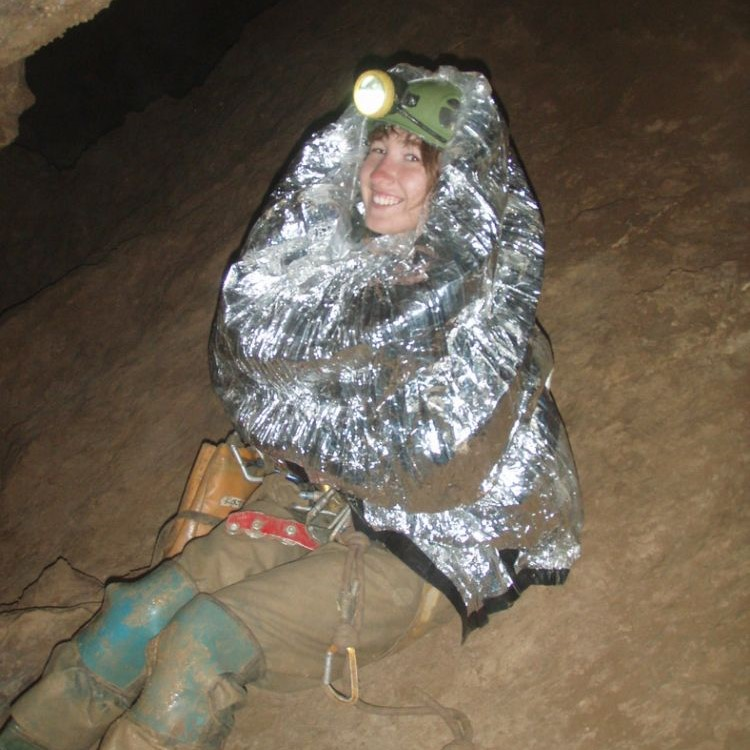
\includegraphics[width=\linewidth]{2011/stories/2011-07-26-11.52.21-Jan Evetts-Olympus Compact-P7260066-Pushing Bolt Traverse on Cheetah--orig_1050p.jpg}}
        \caption{} \label{kate foil}
    \end{subfigure}
    \hfill
     \begin{subfigure}[t]{0.59\textwidth}
        \centering
        \frame{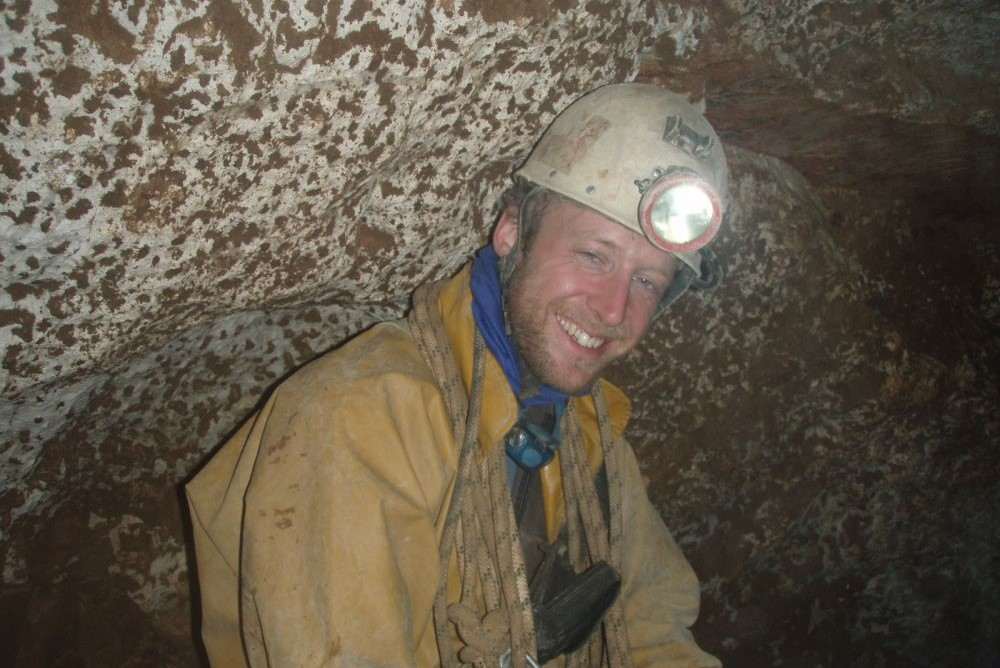
\includegraphics[width=\linewidth]{2011/stories/2011-07-26-17.04.44-Jan Evetts-Olympus Compact-P7260067-Pushing Bolt Traverse on Cheetah--orig_1050p.jpg}}
        \caption{} \label{jan cheetah}
    \end{subfigure}
    
    \vspace{0cm}
    \centering
    \begin{subfigure}[t]{0.59\textwidth}
        \centering
        \frame{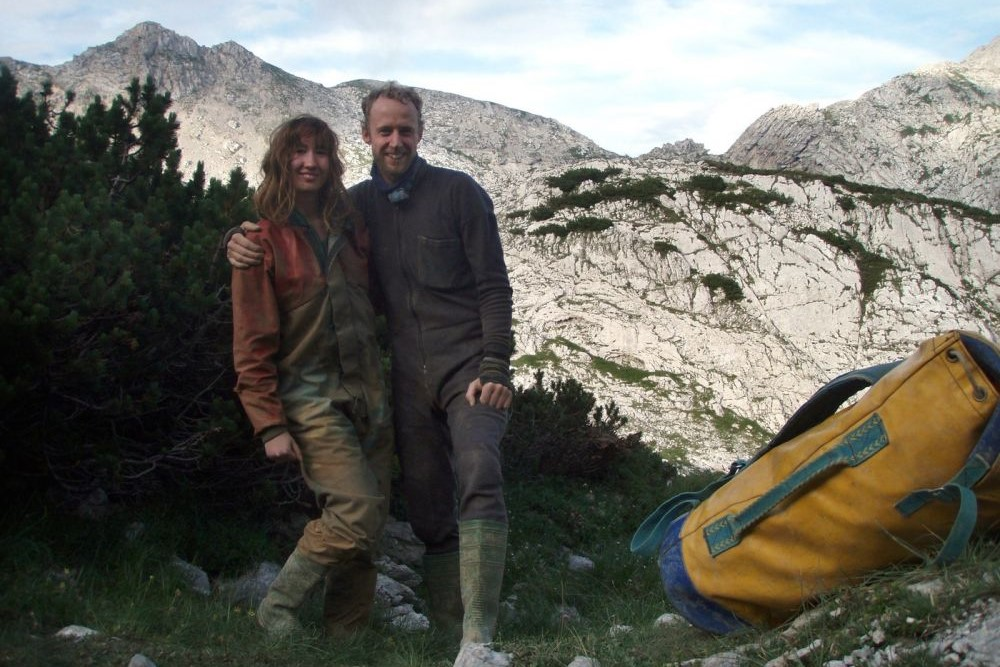
\includegraphics[width=\linewidth]{2011/stories/2011-07-28-17.58.43-Jan Evetts-Olympus Compact-P7280081-Jan and Kates pushing trip--orig_1050p.jpg}}
        \caption{} \label{kate jan}
    \end{subfigure}
    \hfill
    \begin{subfigure}[t]{0.393\textwidth}
        \centering
        \frame{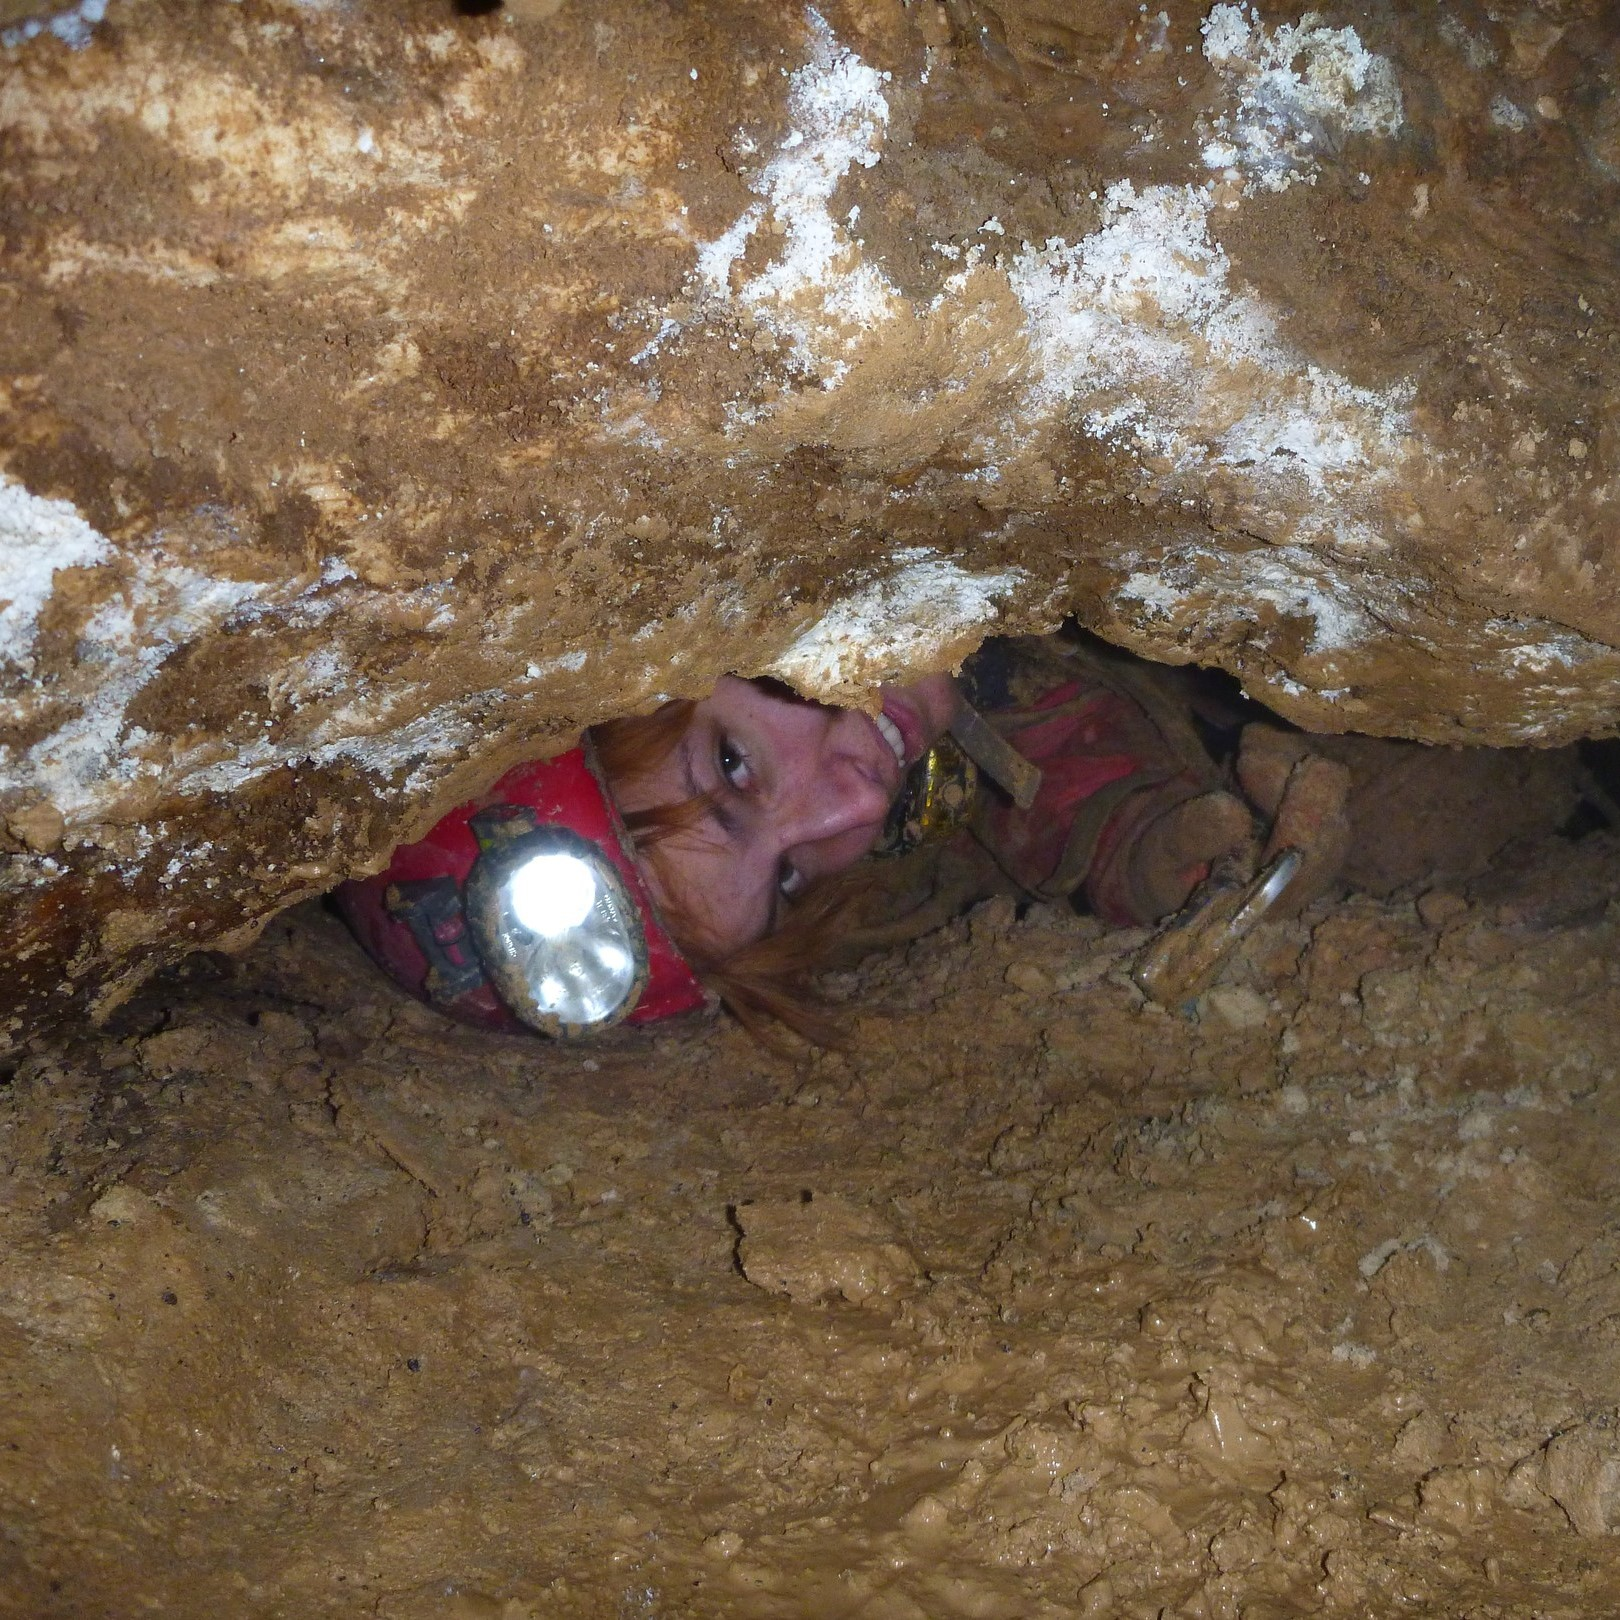
\includegraphics[width=\linewidth]{2011/stories/2011-08-01-19.01.57-Grega-Panasonc DMC-FT2-097-Let Na Drugi Svet--orig.jpg}}
        \caption{} \label{Let Na Drugi Svet 2}
    \end{subfigure}

    \vspace{0cm}
    \begin{subfigure}[t]{\textwidth}
    \centering
        \frame{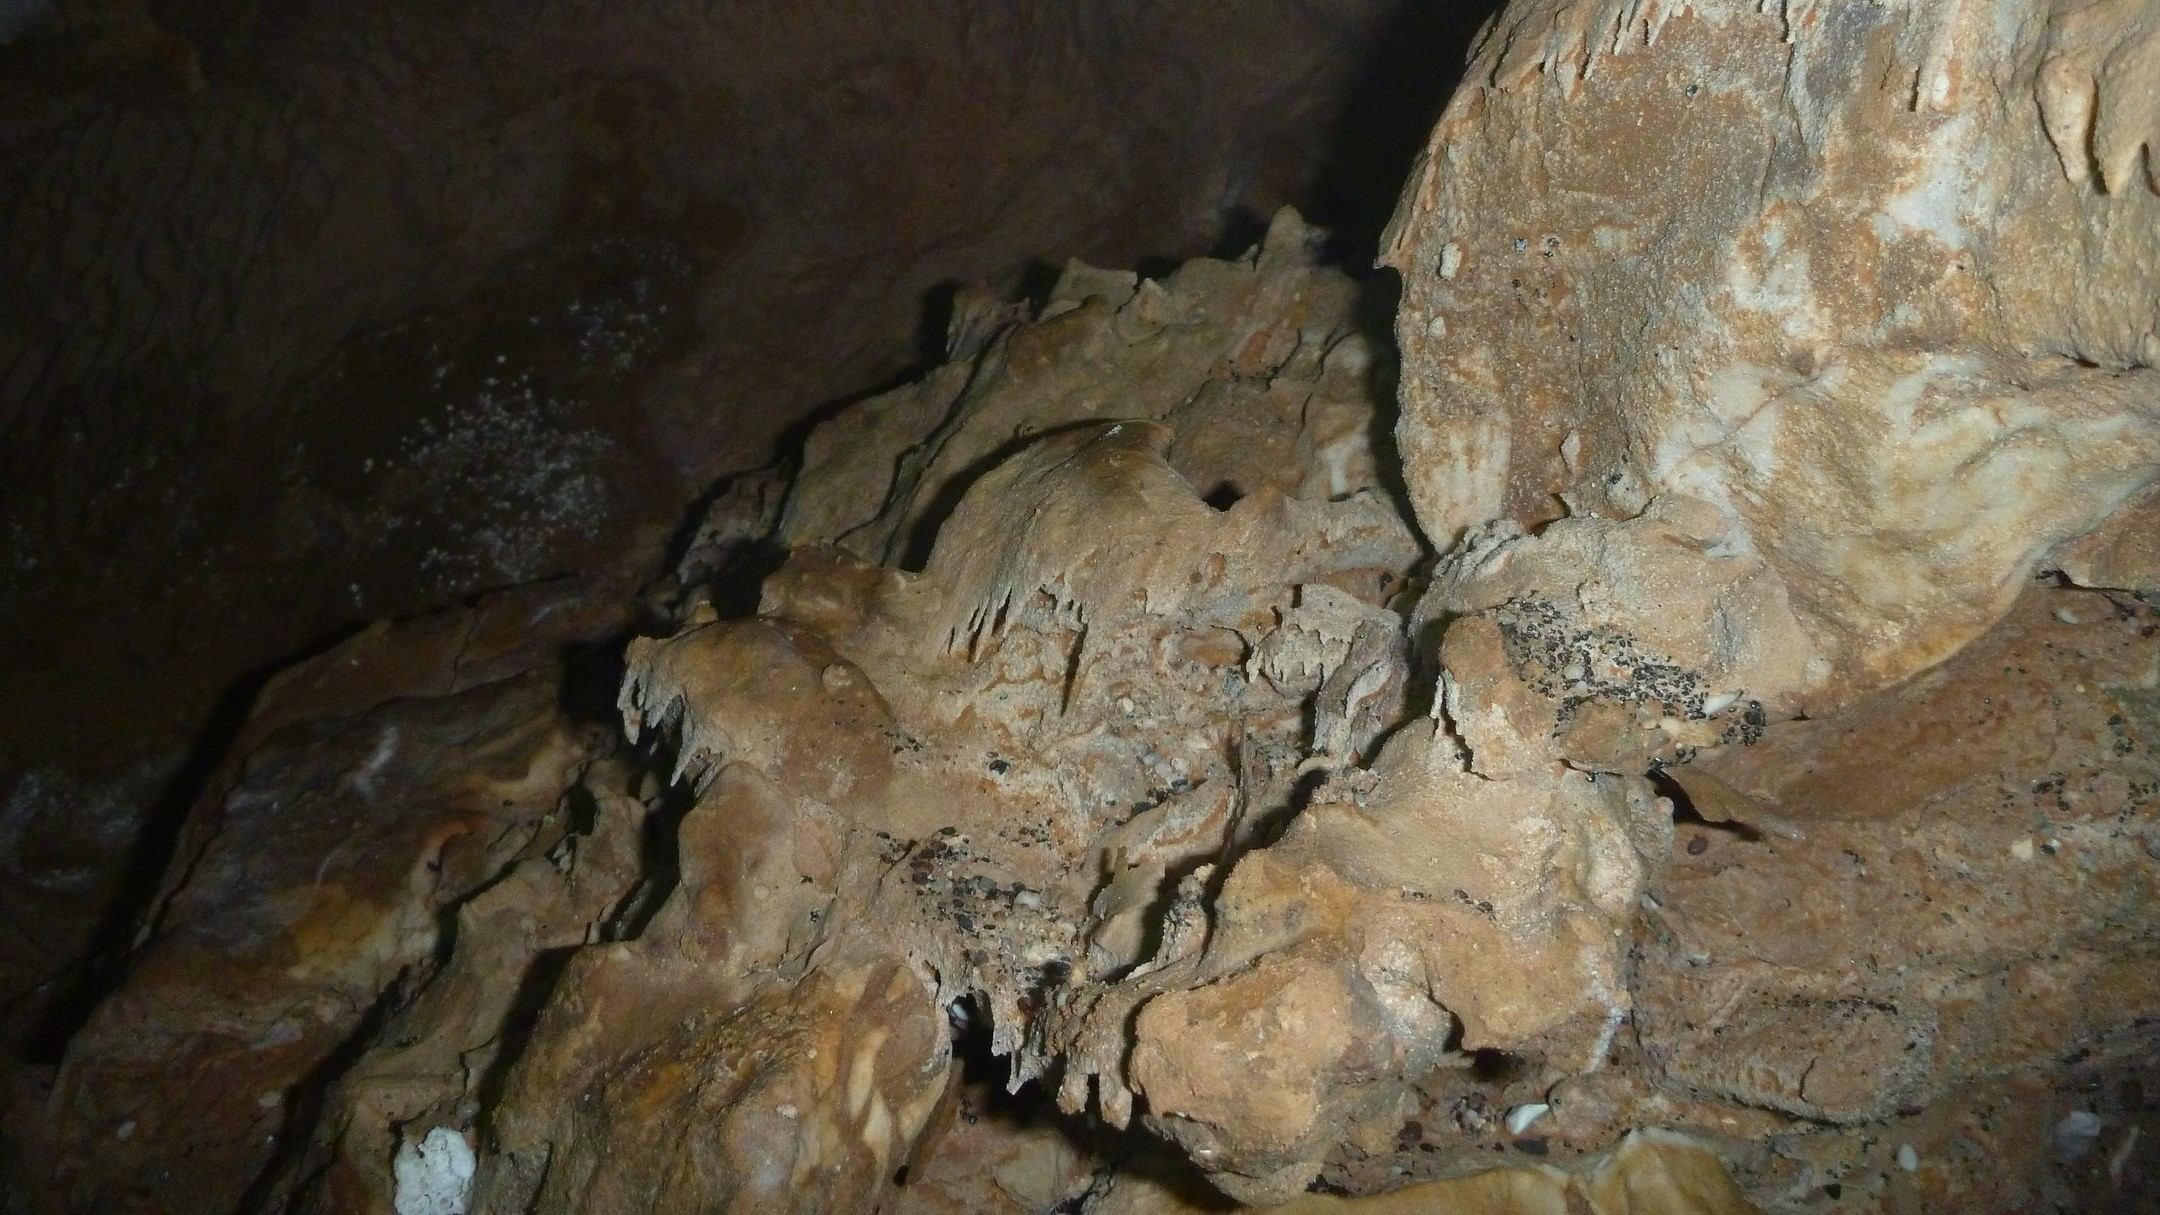
\includegraphics[width=\linewidth]{2011/stories/2011-08-01-18.51.39-Grega-Panasonc DMC-FT2-096-Let Na Drugi Svet--orig.jpg}}
        \caption{} \label{Let Na Drugi Svet 3}
    \end{subfigure}
    \caption{
    \emph{(a)} Kate ensconced in foil as she waits.
    \emph{(b)} Jan pushing the bolt traverse on \passage{Cheetah}.
    \emph{(c)} Kate and Jan on the surface once again. \pic{Jan Evetts / Kate Smith}
    \emph{(d)} Tjaša looking through one of the small dug sections of \passage{Let na Drugi Svet}. 
    \emph{(e)} Not all of \passage{Let na Drugi Svet} is muddy digs. \pic{Grega Maffi}}
\end{pagefigure}


